
\chapter{Introdução}

\section{Contextualização da pesquisa}

Informação de profundidade é uma das representações mais úteis para o entendimento de ambientes físicos \cite{lasinger2019towards} \cite{zhou2019does}. São também uma parte importante da caracterização de relações geométricas de uma determinada cena. As imagens de profundidades (ou mapas de profundidade) desempenham um papel importante em uma série de aplicações que envolvem visão computacional \cite{eigen2014depth}.  Entre elas, podemos citar: compreensão de cenas \cite{jaritz2018sparse}, veículos autônomos \cite{song2021self}, navegação de robôs \cite{ma2019sparse} navegação de VANTs, \cite{padhy2023monocular} fazendas inteligentes \cite{farkhani2019sparse}, e realidade aumentada \cite{du2020depthlab}. 

% \textit{Simultaneos Localization and Mapping} (SLAM) \cite{hu2012robust}

Os mapas de profundidade representam as distâncias de cada ponto (ou pixel) numa cena física em relação ao eixo do dispositivo de captura. Podem ser representados por imagens em escala de cinza, com as cores dos pixels sendo proporcionais à distância, com cinzas mais claros para objetos mais próximos e tons mais escuros para pontos mais afastados (e vice-versa) \cite{dourado2020multi}.

% \begin{figure}[h]
%     \centering
%     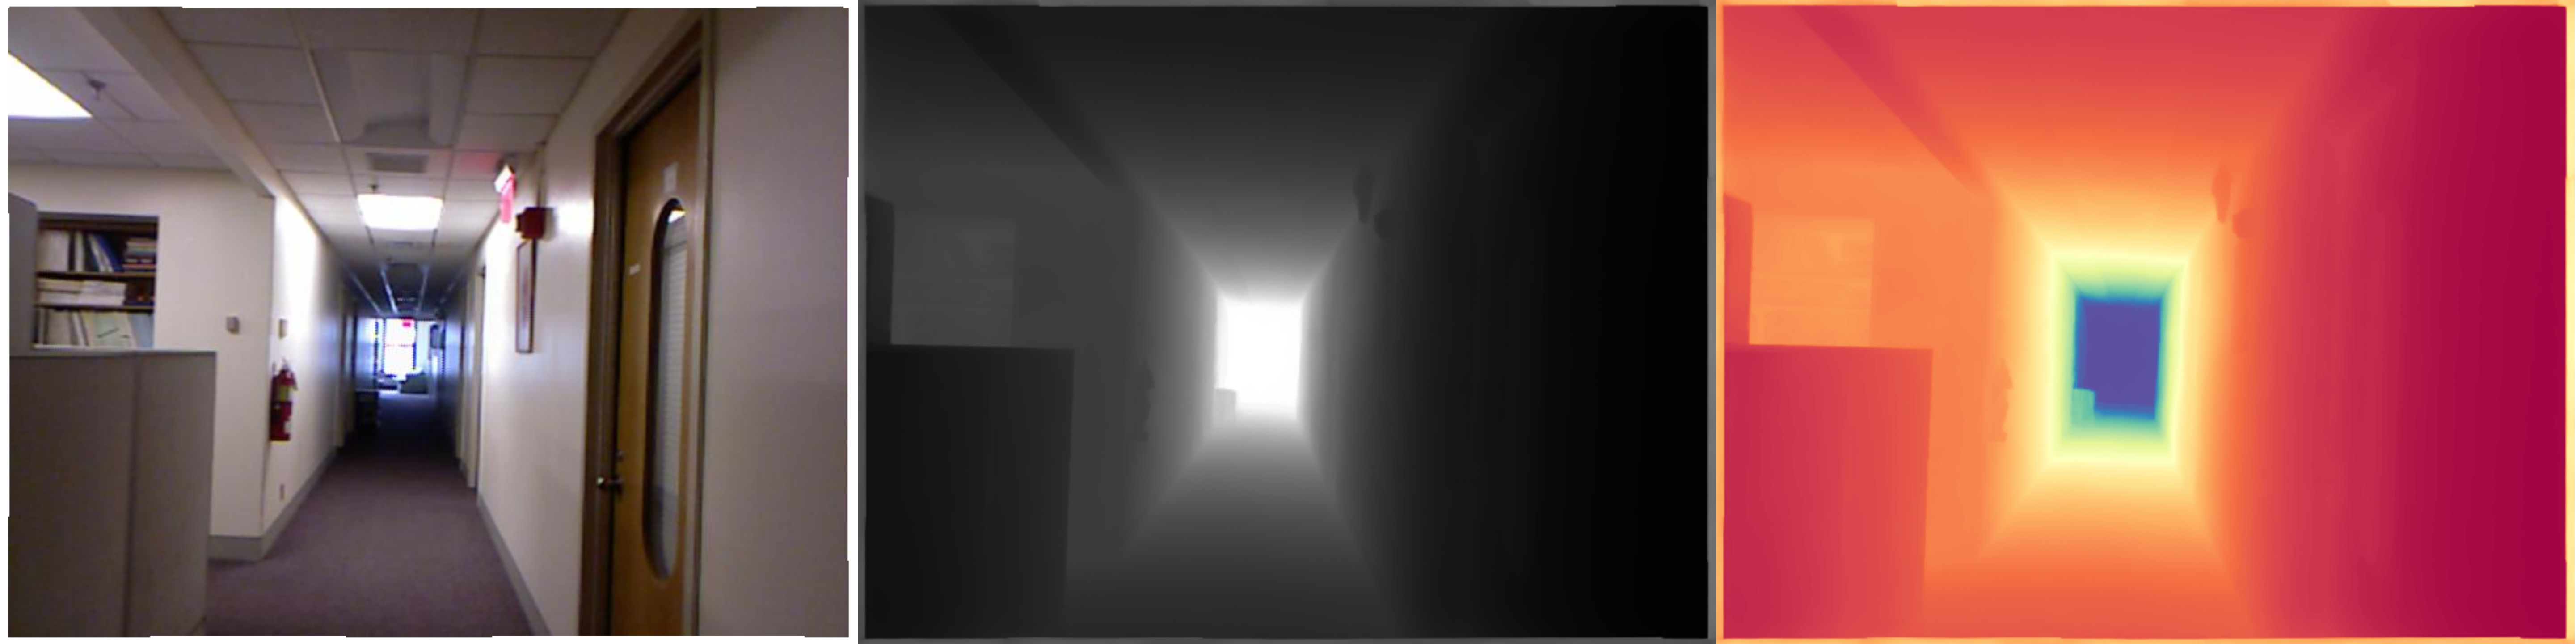
\includegraphics[width=\textwidth]{fig/example_depth.png}
%     \caption{Exemplo de mapa de profundidade do \textit{dataset Nyu Depth V2}. No primeiro quadro, a imagem RGB, no segundo, o mapa de profundidade em escala de cinza, no terceiro uma colorização artificial para o mapa de profundidade.}
%     \label{dmap}
% \end{figure}


Para capturar tais imagens geralmente são empregadas câmeras RGB-D, que podem prover tanto informação de profundidade quanto imagens coloridas da cena. Entre suas tecnologias mais comuns, são encontrados diversos tipos de aquisição que podem ser baseados em visão estereoscópica, que trabalha com múltiplos ângulos de visão, sensores \textit{Time-of-Flight} (ToF) que emprega projeção de lasers infravermelhos (IR) estruturados e técnicas mais precisas como o LiDAR (\textit{Light Detection and Ranging}) \cite{castellano2023performance}.


Sensores de profundidade estão cada vez mais embarcados em equipamentos amplamente difundidos como dispositivos de realidade aumentada (Occulus, Kinnect) e até mesmo em smartphones \cite{du2020depthlab}, principalmente as câmeras ToF, pois são capazes de desempenhar de maneira satisfatória mesmo com baixa potência \cite{branscombe2018microsoft}. De acordo com \cite{xie2021ultradepth}, a adoção de sensores de profundidade em smartphones tende a aumentar nos próximos anos, com diversas aplicações como tradução de linguagem de sinais \cite{park2021enabling} e sistemas de navegação mobile para pessoas com deficiência visual \cite{see2022smartphone}.

%sinal 57, gestos 86, e aumentada 97

Ainda segundo \cite{castellano2023performance}, cada uma das técnicas de aquisição de imagens de profundidade possui lados negativos que podem impactar os dados. Por exemplo, as câmeras ToF podem sofrer com invalidação de pixels próximos a cantos ou bordas de objetos devido à interferências entre os raios IR em superfícies descontínuas ou reflexivas \cite{hansard2012time}. Outros tipos de câmeras RGB-D mais comuns como o Microsoft Kinect ou Intel RealSense podem produzir valores inválidos em superfícies muito brilhantes ou reflexivas como espelhos, superfícies metálicas ou muito escuras \cite{zollhofer2019commodity}. Em ambientes internos, tais imagens podem conter até 50\% de dados faltantes. \cite{zhang2022indepth} \cite{zhang2018deep}. Pontos cuja medição é desconhecida são representados por pixels totalmente pretos ou totalmente brancos \cite{dourado2020multi}.

% \begin{figure}
%     \centering   
%     \includegraphics[width=\textwidth]{fig/depth_problema.png}
%     \caption{Exemplo de imagem RGB com mapa de profundidade apresentando leituras inválidas.}
%     \label{errdepth}
% \end{figure}

%problemas 27, 80, 98

Garantir a correta representação dos mapas em escala de pixel é de considerável importância para as tarefas que dependem de profundidade e que requerem um alto grau de segurança e confiabilidade dos dados, como veículos autônomos ou navegação de drones. A tecnologia LiDAR é a alternativa com implementação mais confiável entre as que foram citadas, no entanto, ressalta-se que nem o LiDAR e nem câmeras RGB-D convencionais produzem mapas completos e densos. No caso do LiDAR, são produzidos mapas esparsos (approx. 95\% de esparsidade) e no caso de câmeras RGB-D ou câmeras ToF são produzidos mapas com partes faltantes em determinadas superfícies ou bordas \cite{hu2012robust}. 




% Neste cenário, tecnologias de aquisição e melhoramento dos dados foram amplamente pesquisadas pela ciência nos últimos anos. Recentemente foram exploradas técnicas que não dependem de sensores de profundidade, ou seja, que inferem a informação de profundidade a partir de uma única imagem RGB capturada a partir de uma câmera comum, essa abordagem é conhecida como \textit{Monocular Depth Estimation} (MDE). No entanto, métodos baseados em características puramente visuais   \cite{szeliski2022computer} \cite{hu2022deep}. 



Considerando as limitações impostas por métodos ativos de aquisição de profundidade, surge a possibilidade de inferir um mapa de profundidade denso e completo de uma cena a partir de uma ou mais imagens RGB, processo conhecido como estimação de profundidade (\textit{Depth Estimation - DE}) \cite{rajapaksha2024deep}. Quando duas imagens de câmeras diferentes são utilizadas para obter-se a informação de profundidade, denomina-se \textit{Stereo Matching (SM)}. No entanto, métodos baseados em imagens \textit{stereo} requerem processos complexos de calibração e alinhamento \cite{dong2022towards}.


O problema da estimação monocular de profundidade (\textit{Monocular Depth Estimation - MDE}) tem por objetivo inferir o mapa de profundidade através de uma única imagem RGB. Esse problema é considerado mal-posto devido à ausência de informação geométrica na projeção da cena 3D para a imagem 2D. No entanto, os avanços nas tecnologias de \textit{Deep Learning - DL} e visão computacional tornaram factível e conveniente o uso de MDE para estimar mapas de profundidade densos e completos. \cite{spencer2024third} \cite{rajapaksha2024deep}. 

Ao longo dos anos, houveram diversas pesquisas científicas abordando o tema de estimação monocular de profundidade utilizando toda a miríade de técnicas e metodologias dentro do universo do DL, empregando desde redes neurais convolucionais \cite{kopf2021robust}, estruturas \textit{encoder-decoder} \cite{godard2019digging}, mistura de bases de dados em grande escala em modos diferentes \cite{lasinger2019towards}, transformadores de visão \cite{birkl2023midas}, modelos de difusão \cite{ke2024repurposing}, e treinamento utilizando dados reais pseudo-rotulados em larga escala \cite{yang2024depth}. 

Neste cenário, este trabalho propõe uma análise comparativa entre os diversos modelos de estimação monocular de profundidade relativa baseados em DL através da abordagem quantitativa, utilizando métricas e \textit{benchmarks} presentes na literatura, abordagem qualitativa e através de uma aplicação.



\section{Motivação e Justificativa} 


 
\section{Objetivos}


\subsection{Objetivo Geral}
Este trabalho possui como objetivo geral a análise comparativa de estimadores monoculares de profundidade robustos capazes de produzir informação de profundidade de alta qualidade para imagens sob quaisquer circunstâncias.

\subsection{Objetivos Específicos}

\begin{itemize}
    \item Estudo e escolha dos datasets que tenha as imagens apropriadas para teste.
    \item Estudo de modelos de estimação monocular de profundidade relativa do estado da arte.
    \item Análise e escolha entre os modelos estudados para implementação e testes.
    \item Implementação de método de pós-processamento para transferência do domínio relativo para métrico baseado em transformação de intensidade.
    \item Avaliação de desempenho perante métricas utilizadas na literatura para comparação entre os modelos no espaço relativo e métrico.
    \item Avaliação qualitativa dos resultados.
    \item Implementação de aplicação com os mapas de profundidade gerados.
    
\end{itemize}

